\documentclass[12pt]{article}%
\usepackage{amsfonts}
\usepackage{fancyhdr}
\usepackage{comment}
\usepackage[a4paper, top=2.5cm, bottom=2.5cm, left=2.2cm, right=2.2cm]%
{geometry}
\usepackage{times}
\usepackage{amsmath}
\usepackage{changepage}
\usepackage{amssymb}
\usepackage{graphicx}%

\usepackage{listings}
\usepackage{color}

\definecolor{dkgreen}{rgb}{0,0.6,0}
\definecolor{gray}{rgb}{0.5,0.5,0.5}
\definecolor{mauve}{rgb}{0.58,0,0.82}

\lstset{frame=tb,
  language=Python,
  aboveskip=3mm,
  belowskip=3mm,
  showstringspaces=false,
  columns=flexible,
  basicstyle={\small\ttfamily},
  numbers=none,
  numberstyle=\tiny\color{gray},
  keywordstyle=\color{blue},
  commentstyle=\color{dkgreen},
  stringstyle=\color{mauve},
  breaklines=true,
  breakatwhitespace=true,
  tabsize=4
}

\setcounter{MaxMatrixCols}{30}
\newtheorem{theorem}{Theorem}
\newtheorem{acknowledgement}[theorem]{Acknowledgement}
\newtheorem{algorithm}[theorem]{Algorithm}
\newtheorem{axiom}{Axiom}
\newtheorem{case}[theorem]{Case}
\newtheorem{claim}[theorem]{Claim}
\newtheorem{conclusion}[theorem]{Conclusion}
\newtheorem{condition}[theorem]{Condition}
\newtheorem{conjecture}[theorem]{Conjecture}
\newtheorem{corollary}[theorem]{Corollary}
\newtheorem{criterion}[theorem]{Criterion}
\newtheorem{definition}[theorem]{Definition}
\newtheorem{example}[theorem]{Example}
\newtheorem{exercise}[theorem]{Exercise}
\newtheorem{lemma}[theorem]{Lemma}
\newtheorem{notation}[theorem]{Notation}
\newtheorem{problem}[theorem]{Problem}
\newtheorem{proposition}[theorem]{Proposition}
\newtheorem{remark}[theorem]{Remark}
\newtheorem{solution}[theorem]{Solution}
\newtheorem{summary}[theorem]{Summary}
\newenvironment{proof}[1][Proof]{\textbf{#1.} }{\ \rule{0.5em}{0.5em}}

\newcommand{\Q}{\mathbb{Q}}
\newcommand{\R}{\mathbb{R}}
\newcommand{\C}{\mathbb{C}}
\newcommand{\Z}{\mathbb{Z}}

\begin{document}

\title{CS 498: Computational Advertising \\
       Homework 4}
\author{Zhenye Na (zna2)}
\date{\today}
\maketitle



\section{Part 1 - Reading Assignment}


\subsection{Selected Subtopic}

Advances driven by Artificial Intelligence

\subsubsection{main idea/issue/problem statement of this topic in one sentence}

Online advertising often involves highly complex, contingency-based decision-making processes to determine what type of digital content to send to which audience segments when various event contingencies occur and is heightened in the political context, as individual sentiments about political ideas or candidates are often particularly impressionable and therefore fickle.

\subsubsection{why is the problem hard?}

This confluence of AI-driven technology and advertising practice means that even poorly executed disinformation campaigns will achieve results because they will benefit from similar, better ones that have taught the algorithms. Their targeting efforts were reportedly unsophisticated; they simply took advantage of the basic tools of today’s information markets that are designed to deliver targeted persuasive messages to tens of millions of people at low cost and with little transparency.

\subsubsection{why is the problem interesting?}

AI excels at finding patterns and insights from data—patterns and insights that humans find difficult or impossible to see. This makes AI perfect for augmenting paid advertising activities. AI systems can inhale data on ad performance and effectiveness, then use that data to adjust campaign specifics accordingly. This topic is very promising since the Artificial Intelligence is more and more popular right now.


\subsubsection{what interests you specifically about this problem in one sentence}

AI and its associated family of advanced algorithmic technologies are thus likely to play an enlarged role in the context of political disinformation propagated through online social platforms, which is promising in future.


\subsection{Selected Research paper}

Artificial Intelligence in Advertising - How Marketers Can Leverage Artificial Intelligence Along the Consumer Journey, \textit{Journal of Advertising Research}, Jan Kietzmann, Jeannette Paschen, Emily Treen

\subsubsection{State in one sentence the main idea of this paper.}

Marketers are turning to artificial intelligence (AI) to transform this (big) data flow into valuable consumer insight. 

\subsubsection{Mention three strengths of this paper.}

\begin{enumerate}
\item AI-enabled search results, ad targeting and Predictive modeling (potential customer)
\item Predictive lead scoring, Content curation, Emotion AI
\item “Intelligent” purchasing, Dynamic pricing and Ad retargeting
\end{enumerate}


\subsubsection{Mention three weakness of this paper.}

\begin{enumerate}
\item risks involved, such as outcomes related to Cambridge Analytica’s historic use of millions of Facebook accounts for political purposes
\item “dark side” of data mining and the use of AI in analyzing and managing social-media data
\item must adapt the AI systems to comply with new privacy standards. 
\end{enumerate}

\subsubsection{Suggest one improvement over the paper.}

Instead of just saying "AI can improve marketing/advertising", add some real world campaign example to illustrate these ideas.


\subsection{Selected News Article 1}

The value of applying artificial intelligence in display advertising, \textit{Adam Grow}.

\subsubsection{State in one sentence the main idea of this News Article.}

Artificial super-intelligence will cause such rapid growth that human civilization will experience incomprehensible change, which affects the way we interact with brands and the experiences that lead us to purchase.

\subsubsection{Mention three strengths of this News Article.}

\begin{enumerate}
\item AI provides efficiency in campaign management
\item AI allows marketers to more efficiently drive performance through relevant and personalized advertisements that leverage enhanced targeting algorithms and creative optimization
\item AI is a conduit for relevant and personalized experiences
\end{enumerate}


\subsubsection{Mention three weakness of this News Article.}

\begin{enumerate}
\item human touch in campaign management remains imperative
\item there are still pieces that can only be recognized and managed by a human
\item technology must continue to evolve for brands to deliver powerful ad experiences among changing consumer behaviors, platforms and media.
\end{enumerate}


\subsubsection{Suggest one improvement over the News Article.}

This news article describe AI in advertising thouroughtly, which is really enjoyable for people who come from AI field. However, there is not so much background info concerning Advertising aspect.


\subsection{Selected News Article 2}

\subsubsection{State in one sentence the main idea of this News Article.}

How Artificial Intelligence Can Supercharge Your Paid Advertising, \textit{Mike Kaput}


\subsubsection{Mention three strengths of this News Article.}

\begin{enumerate}
\item competitive intelligence
\item campaign optimization
\item lightning-fast multitasking at high speeds
\end{enumerate}


\subsubsection{Mention three weakness of this News Article.}

\begin{enumerate}
\item Marketers must learn how to work hand-in-hand with intelligent tools and systems. This requires a solid understanding of what’s possible with artificial intelligence—and where AI systems can be most profitably used to augment activities.
\item require marketers to change
\item need to be used properly
\end{enumerate}


\subsubsection{Suggest one improvement over the News Article.}

This article illustrate greatly on the influence of marketer when AI in advertising is more and more useful, if more information like the platform of existing AI can be provided.


\subsection{Conclusion : Briefly state the main lesson learned about the topic after reading these three contents.}

Artificial intelligence is the science of making machines smart, to augment and assist human activities. In marketing, AI excels at finding patterns and insights from data—patterns and insights that humans find difficult or impossible to see. 


\section{Part 2 - Advertisement Analysis}

\subsection{Code}

\begin{lstlisting}
import os
import json
import requests

from PIL import Image
from io import BytesIO

# read json file to python dictionary
json_file = open('../ads.json')
json_str = json_file.read()
json_data = json.loads(json_str)
ads = json_data["ads"]

# filter out ads containing keyword logo in their url
selected_ads = []
for visited_page_url, ad_urls in ads.items():
    # list of ads str
    if isinstance(ad_urls, list):
        for ad_url in ad_urls:
            if ad_url.find("logo") == -1:
                selected_ads.append(ad_url)
    # ads strs
    elif isinstance(ad_urls, str):
        if ad_url.find("logo") == -1:
            selected_ads.append(ad_url)

# download images
for idx, url in enumerate(selected_ads):
    response = requests.get(url, stream=True)
    try:
        image = Image.open(BytesIO(response.content))
        width, height = image.size
        if width > 1 and height > 1:
            # images.append(image)
            image.save("{}th_ad.png".format(idx))
    except:
        continue
\end{lstlisting}


\subsection{Advertisement Analysis}

ontology: gender, ethnicity, location, career, age, education, marriage, price, season, social

118 images total, 56 of them are legitimate.


\subsection{Bar Chart}

\[
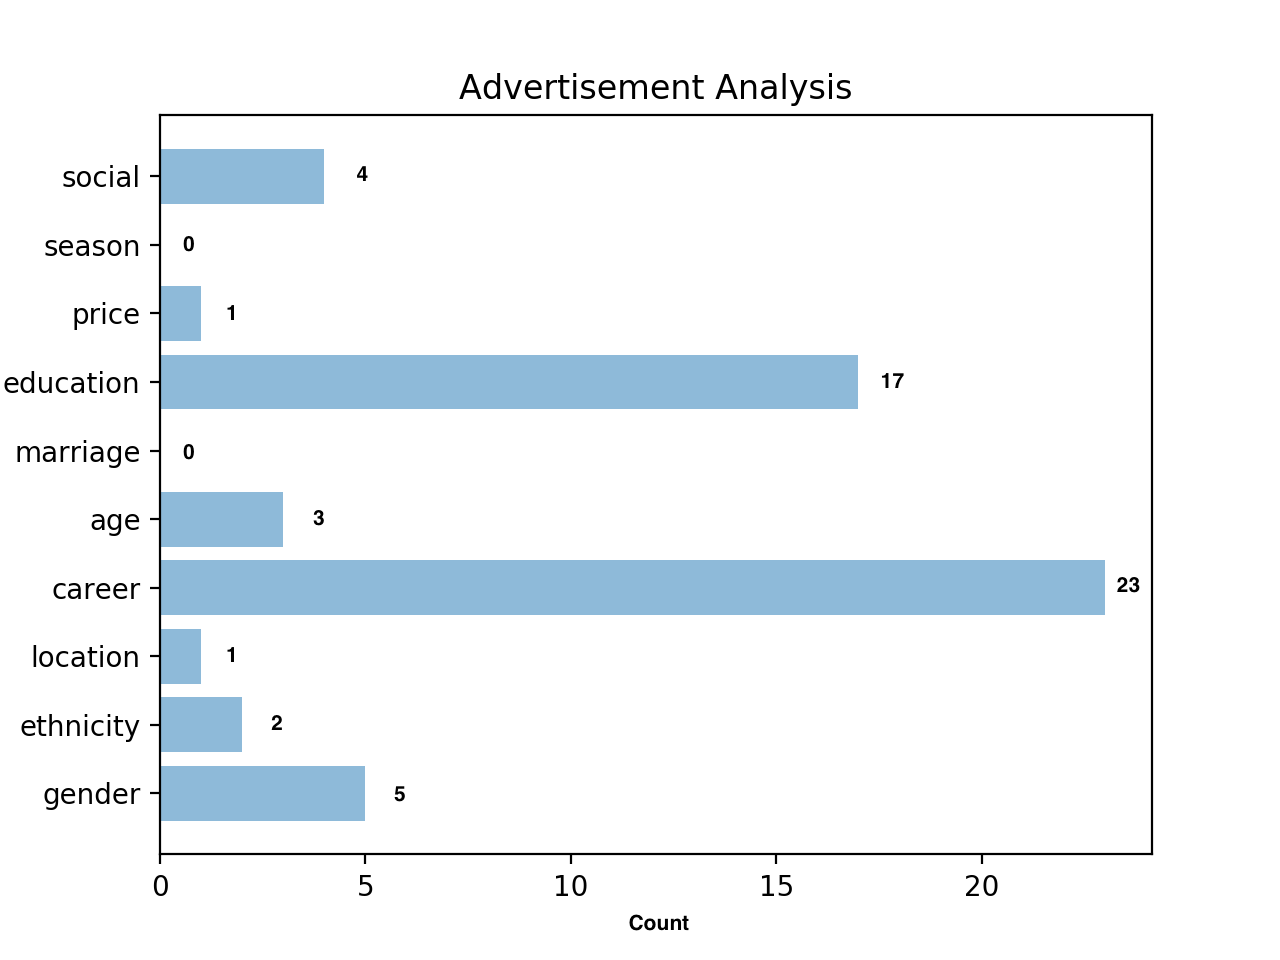
\includegraphics{Figure_1.png}
\]



\end{document}